%-----------------------------------------------------------------------------------------------------------------------------------------------%
%	The MIT License (MIT)
%
%	Copyright (c) 2019 Jan Küster
%
%	Permission is hereby granted, free of charge, to any person obtaining a copy
%	of this software and associated documentation files (the "Software"), to deal
%	in the Software without restriction, including without limitation the rights
%	to use, copy, modify, merge, publish, distribute, sublicense, and/or sell
%	copies of the Software, and to permit persons to whom the Software is
%	furnished to do so, subject to the following conditions:
%	
%	THE SOFTWARE IS PROVIDED "AS IS", WITHOUT WARRANTY OF ANY KIND, EXPRESS OR
%	IMPLIED, INCLUDING BUT NOT LIMITED TO THE WARRANTIES OF MERCHANTABILITY,
%	FITNESS FOR A PARTICULAR PURPOSE AND NONINFRINGEMENT. IN NO EVENT SHALL THE
%	AUTHORS OR COPYRIGHT HOLDERS BE LIABLE FOR ANY CLAIM, DAMAGES OR OTHER
%	LIABILITY, WHETHER IN AN ACTION OF CONTRACT, TORT OR OTHERWISE, ARISING FROM,
%	OUT OF OR IN CONNECTION WITH THE SOFTWARE OR THE USE OR OTHER DEALINGS IN
%	THE SOFTWARE.
%	
%
%-----------------------------------------------------------------------------------------------------------------------------------------------%


%============================================================================%
%
%	DOCUMENT DEFINITION
%
%============================================================================%

%we use article class because we want to fully customize the page and don't use a cv template
\documentclass[10pt,A4]{article}	


%----------------------------------------------------------------------------------------
%	ENCODING
%----------------------------------------------------------------------------------------

% we use utf8 since we want to build from any machine
\usepackage[utf8]{inputenc}		
%----------------------------------------------------------------------------------------
%	LOGIC
%----------------------------------------------------------------------------------------

% provides \isempty test
\usepackage{xstring, xifthen}

%----------------------------------------------------------------------------------------
%	FONT BASICS
%----------------------------------------------------------------------------------------

% some tex-live fonts - choose your own

%\usepackage[defaultsans]{droidsans}
%\usepackage[default]{comfortaa}
%\usepackage{cmbright}
\usepackage[default]{raleway}
%\usepackage{fetamont}
%\usepackage[default]{gillius}
%\usepackage[light,math]{iwona}
%\usepackage[thin]{roboto} 

% set font default
\renewcommand*\familydefault{\sfdefault} 	
\usepackage[T1]{fontenc}

% more font size definitions
\usepackage{moresize}

%----------------------------------------------------------------------------------------
%	FONT AWESOME ICONS
%---------------------------------------------------------------------------------------- 

% include the fontawesome icon set
\usepackage{fontawesome}

% use to vertically center content
% credits to: http://tex.stackexchange.com/questions/7219/how-to-vertically-center-two-images-next-to-each-other
\newcommand{\vcenteredinclude}[1]{\begingroup
\setbox0=\hbox{\includegraphics{#1}}%
\parbox{\wd0}{\box0}\endgroup}

% use to vertically center content
% credits to: http://tex.stackexchange.com/questions/7219/how-to-vertically-center-two-images-next-to-each-other
\newcommand*{\vcenteredhbox}[1]{\begingroup
\setbox0=\hbox{#1}\parbox{\wd0}{\box0}\endgroup}

% icon shortcut
\newcommand{\icon}[3] { 							
	\makebox(#2, #2){\textcolor{maincol}{\csname fa#1\endcsname}}
}	

% icon with text shortcut
\newcommand{\icontext}[4]{ 						
	\vcenteredhbox{\icon{#1}{#2}{#3}}  \hspace{2pt}  \parbox{0.9\mpwidth}{\textcolor{#4}{#3}}
}

% icon with website url
\newcommand{\iconhref}[5]{ 						
    \vcenteredhbox{\icon{#1}{#2}{#5}}  \hspace{2pt} \href{#4}{\textcolor{#5}{#3}}
}

% icon with email link
\newcommand{\iconemail}[5]{ 						
    \vcenteredhbox{\icon{#1}{#2}{#5}}  \hspace{2pt} \href{mailto:#4}{\textcolor{#5}{#3}}
}

%----------------------------------------------------------------------------------------
%	PAGE LAYOUT  DEFINITIONS
%----------------------------------------------------------------------------------------

% page outer frames (debug-only)
% \usepackage{showframe}		

% we use paracol to display breakable two columns
\usepackage{paracol}

% define page styles using geometry
\usepackage[a4paper]{geometry}

% remove all possible margins
\geometry{top=1cm, bottom=1cm, left=1cm, right=1cm}

\usepackage{fancyhdr}
\pagestyle{empty}

% space between header and content
% \setlength{\headheight}{0pt}

% indentation is zero
\setlength{\parindent}{0mm}

%----------------------------------------------------------------------------------------
%	TABLE /ARRAY DEFINITIONS
%---------------------------------------------------------------------------------------- 

% extended aligning of tabular cells
\usepackage{array}

% custom column right-align with fixed width
% use like p{size} but via x{size}
\newcolumntype{x}[1]{%
>{\raggedleft\hspace{0pt}}p{#1}}%


%----------------------------------------------------------------------------------------
%	GRAPHICS DEFINITIONS
%---------------------------------------------------------------------------------------- 

%for header image
\usepackage{graphicx}

% use this for floating figures
% \usepackage{wrapfig}
% \usepackage{float}
% \floatstyle{boxed} 
% \restylefloat{figure}

%for drawing graphics		
\usepackage{tikz}				
\usetikzlibrary{shapes, backgrounds,mindmap, trees}

%----------------------------------------------------------------------------------------
%	Color DEFINITIONS
%---------------------------------------------------------------------------------------- 
\usepackage{transparent}
\usepackage{color}

% primary color
\definecolor{maincol}{RGB}{40, 122, 138}

% accent color, secondary
% \definecolor{accentcol}{RGB}{ 250, 150, 10 }

% dark color
\definecolor{darkcol}{RGB}{107, 46, 69}

% light color
\definecolor{lightcol}{RGB}{100, 201, 167}


% Package for links, must be the last package used
\usepackage[hidelinks]{hyperref}

% returns minipage width minus two times \fboxsep
% to keep padding included in width calculations
% can also be used for other boxes / environments
\newcommand{\mpwidth}{\linewidth-\fboxsep-\fboxsep}
	


%============================================================================%
%
%	CV COMMANDS
%
%============================================================================%

%----------------------------------------------------------------------------------------
%	 CV LIST
%----------------------------------------------------------------------------------------

% renders a standard latex list but abstracts away the environment definition (begin/end)
\newcommand{\cvlist}[1] {
	\begin{itemize}{#1}\end{itemize}
}

%----------------------------------------------------------------------------------------
%	 CV TEXT
%----------------------------------------------------------------------------------------

% base class to wrap any text based stuff here. Renders like a paragraph.
% Allows complex commands to be passed, too.
% param 1: *any
\newcommand{\cvtext}[1] {
	\begin{tabular*}{1\mpwidth}{p{0.98\mpwidth}}
		\parbox{1\mpwidth}{#1}
	\end{tabular*}
}

%----------------------------------------------------------------------------------------
%	CV SECTION
%----------------------------------------------------------------------------------------

% Renders a a CV section headline with a nice underline in main color.
% param 1: section title
\newcommand{\cvsection}[1] {
	\vspace{14pt}
	\cvtext{
		\textbf{\LARGE{\textcolor{darkcol}{\uppercase{#1}}}}\\[-4pt]
		\textcolor{maincol}{ \rule{0.1\textwidth}{2pt} } \\
	}
}

%----------------------------------------------------------------------------------------
%	META SKILL
%----------------------------------------------------------------------------------------

% Renders a progress-bar to indicate a certain skill in percent.
% param 1: name of the skill / tech / etc.
% param 2: level (for example in years)
% param 3: percent, values range from 0 to 1
\newcommand{\cvskill}[3] {
	\begin{tabular*}{1\mpwidth}{p{0.72\mpwidth}  r}
 		\textcolor{black}{\textbf{#1}} & \textcolor{maincol}{#2}\\
	\end{tabular*}%
	
	\hspace{4pt}
	\begin{tikzpicture}[scale=1,rounded corners=2pt,very thin]
		\fill [lightcol] (0,0) rectangle (1\mpwidth, 0.15);
		\fill [maincol] (0,0) rectangle (#3\mpwidth, 0.15);
  	\end{tikzpicture}%
}


%----------------------------------------------------------------------------------------
%	 CV EVENT
%----------------------------------------------------------------------------------------

% Renders a table and a paragraph (cvtext) wrapped in a parbox (to ensure minimum content
% is glued together when a pagebreak appears).
% Additional Information can be passed in text or list form (or other environments).
% the work you did
% param 1: time-frame i.e. Sep 14 - Jan 15 etc.
% param 2:	 event name (job position etc.)
% param 3: Customer, Employer, Industry
% param 4: Short description
% param 5: work done (optional)
% param 6: technologies include (optional)
% param 7: achievements (optional)
\newcommand{\cvevent}[5] {
	
	% we wrap this part in a parbox, so title and description are not separated on a pagebreak
	% if you need more control on page breaks, remove the parbox
	\parbox{\mpwidth}{
		\begin{tabular*}{1\mpwidth}{p{0.72\mpwidth}  r}
	 		\textcolor{black}{\textbf{#2}} & \colorbox{maincol}{\makebox[0.25\mpwidth]{\textcolor{white}{#1}}} \\
			\textcolor{maincol}{\textbf{#3}} & \\
		\end{tabular*}\\[8pt]
	
		\ifthenelse{\isempty{#4}}{}{
			\cvtext{#4}\\
		}
	}
}

%----------------------------------------------------------------------------------------
%	 CV META EVENT
%----------------------------------------------------------------------------------------

% Renders a CV event on the sidebar
% param 1: title
% param 2: subtitle (optional)
% param 3: customer, employer, etc,. (optional)
% param 4: info text (optional)
\newcommand{\cvmetaevent}[4] {
	\textcolor{maincol} {\cvtext{\textbf{\begin{flushleft}#1\end{flushleft}}}}

	\ifthenelse{\isempty{#2}}{}{
	\textcolor{darkcol} {\cvtext{\textbf{#2}} }
	}

	\ifthenelse{\isempty{#3}}{}{
		\cvtext{{ \textcolor{darkcol} {#3} }}\\
	}

	\cvtext{#4}\\[14pt]
}

%---------------------------------------------------------------------------------------
%	QR CODE
%----------------------------------------------------------------------------------------

% Renders a qrcode image (centered, relative to the parentwidth)
% param 1: percent width, from 0 to 1
\newcommand{\cvqrcode}[1] {
	\begin{center}
		
\includegraphics[width={#1}\mpwidth]{qrcode}
	\end{center}
}


%============================================================================%
%
%
%
%	DOCUMENT CONTENT
%
%
%
%============================================================================%
\begin{document}
\section{}
\columnratio{0.31}
\setlength{\columnsep}{2.2em}
\setlength{\columnseprule}{4pt}
\colseprulecolor{lightcol}
\begin{paracol}{2}
\begin{leftcolumn}
%---------------------------------------------------------------------------------------
%	META IMAGE
%----------------------------------------------------------------------------------------
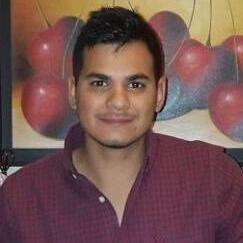
\includegraphics[width=\linewidth]{Foto_CV.png}	%trimming relative to image size

%---------------------------------------------------------------------------------------
%	META SKILLS
%----------------------------------------------------------------------------------------

\cvsection{HABILIDADES}

\cvskill{Python} {5+ yrs} {1} \\[-2pt]

\cvskill{C++} {7+ yrs} {0.9} \\[-2pt]

\cvskill{LAMP/WAMP} {4+ yrs} {0.85} \\[-2pt]

\cvskill{Google Analytics} {2+ yrs} {0.75} \\[-2pt]

\cvskill{Selenium/Docker} {2+ yrs} {0.75} \\[-2pt]

\cvskill{Django/Dash} {2+ yrs} {0.8} \\[-2pt]

\cvskill{HTML/CSS/Markdown} {5+ yrs} {0.9} \\[-2pt]

\cvskill{Javascript/PHP} {5+ yrs} {0.85} \\[-2pt]

\cvskill{Fortran} {8+ yrs} {0.9} \\[-2pt]

\cvskill{Visual Basic} {8+ yrs} {0.8} \\[-2pt]

\cvskill{R} {5+ yrs} {1} \\[-2pt]

\cvskill{Matlab} {5+ yrs} {1} \\[-2pt]

\cvskill{GitHub} {5+ yrs} {1} \\[-2pt]

\cvsection{CONTACTO}

\icontext{MapMarker}{12}{Hermosillo, Sonora}{black}\\[6pt]
\icontext{MobilePhone}{12}{662-364-8525}{black}\\[6pt]
\iconemail{Envelope}{12}{alan.matzumiya@gmail.com}{alan.matzumiya@gmail.com}{black}\\[6pt]
\iconhref{Github}{12}{github.com/alanmatzumiya}{https://github.com/alanmatzumiya}{black}\\[6pt]

%---------------------------------------------------------------------------------------
%	EDUCATION
%---------------------------------------------------------------------------------------- 
\cvsection{IDIOMAS}

\cvskill{Ingl\'es Oral}{80 \%}{0.8} \\[-2pt]
\cvskill{Ingl\'es Escrito}{90 \%}{0.9} \\[-2pt]

\cvsection{EDUCACI\'ON}

\cvmetaevent
{2011 - 2016}
{Ingenier\'ia Qu\'imica}
{Universidad de Sonora}
{Titulado mediante la presentaci\'on de tesis, la cual se desarroll\'o en el \'area de materiales bajo el tema de: \\
	
\href{http://www.repositorioinstitucional.uson.mx/handle/unison/1840}{\textbf{Caracterizaci\'on y evaluaci\'on de las propiedades bioactivas de una mezcla de biocomp\'ositos de hidroxiapatita/$\beta$-wollastonita preparados por el m\'etodo sol gel: sometidos a tratamientos t\'ermicos diferentes}}.}

\cvmetaevent
{2017 - 2019}
{Maestr\'ia en Ciencias Matem\'aticas}
{Universidad de Sonora}
{El objetivo para obtener este grado fue desarrollar fuertes conocimientos en el \'area del an\'alisis num\'erico, los cuales me permitieron elaborar un trabajo de tesis acerca de los m\'etodos espectrales haciendo uso de las transformadas de Fourier para resolver ecuaciones diferenciales parciales que se presentan en din\'amica de fluidos. Mi trabajo de tesis, junto con los c\'odigos que he desarrollado para entender su implementaci\'on computacional, pueden ser consultados en:

\href{https://github.com/alanmatzumiya/spectral-methods}{\textbf{gh-pages/spectral-methods}}.}

\vfill\null

%---------------------------------------------------------------------------------------
%	CERTIFICATION
%----------------------------------------------------------------------------------------
  

\end{leftcolumn}
\begin{rightcolumn}
%---------------------------------------------------------------------------------------
%	TITLE  HEADER
%----------------------------------------------------------------------------------------
\label{spanish}
\cvskill{} {\hyperref[english]{Leer en Ingl\'es}} {1} \\[2pt]
\fcolorbox{white}{darkcol}{\begin{minipage}[c][3.5cm][c]{1\mpwidth}
	\begin {center}
		\HUGE{ \textbf{ \textcolor{white}{ \uppercase{ Alan Daniel Matzumiya Zazueta } } } } \\[-24pt]
		\textcolor{white}{ \rule{0.1\textwidth}{1.25pt} } \\[4pt]
		\large{ \textcolor{white} {Ingeniero Qu\'imico y Maestro en Ciencias Matem\'aticas.} }
 	\end {center}
\end{minipage}} \\[14pt]
\vspace{-12pt}

%---------------------------------------------------------------------------------------
%	PROFILE
%----------------------------------------------------------------------------------------
\vspace{12mm}
\cvsection{SOBRE MI}
\\
\cvtext{\textbf{Edad:} 27 años  \hspace{2mm}  \textbf{Fecha de Nacimiento:} 14/09/1992}
\\\\
\cvtext{\textbf{Lugar de Nacimiento:} Guaymas, Son. \textbf{Residencia Actual:} Hermosillo, Son.}
\\\\
\cvtext{Gracias a mi formación acad\'emica, me ha sido posible obtener una amplia variedad de herramientas matem\'aticas que me permiten plantear y desarrollar problemas que requieren interpretaci\'on a trav\'es de modelos que pueden ser \'utiles en funci\'on de su finalidad. \\

Por iniciativa propia, y de forma autodidacta, practico en diferentes lenguajes de programaci\'on, los cuales he utilizado no solo con fines matem\'aticos sino que tambi\'en he logrado obtener buenas experiencias en el desarrollo web y de aplicaciones. \\

Mi principal inter\'es es profundizar en el \'area de an\'alisis de datos, que con mis habilidades en matem\'aticas me ha sido posible explorar, interpretar y trabajar con datos utilizando \textbf{Python}, siendo este el lenguaje de programaci\'on que más domino debido a la pr\'actica constante que he realizado para mi formaci\'on como programador. \\
\vspace{0.5cm}

\fcolorbox{white}{darkcol}{\begin{minipage}[c][1cm][c]{1\mpwidth}
	\begin {center}
		\large{ \textcolor{white} {Si deseas saber m\'as sobre m\'i, puedes visitar mi sitio web:  }}
		\\[4pt]
		\large{ \textcolor{white} {
\hyperlink{https://alanmatzumiya.github.io/}{\textbf{https://alanmatzumiya.github.io}}} }
 	\end {center}
\end{minipage}}
\\\\
Aqu\'i puedes encontrar proyectos e informaci\'on m\'as detallada sobre mi formaci\'on acad\'emica y profesional.
}

%---------------------------------------------------------------------------------------
%	WORK EXPERIENCE
%----------------------------------------------------------------------------------------
\vspace{5mm}
\cvsection{Experencia Laboral}

\cvevent
{mayo - junio 2015}
{Practicas Profesionales}
{CFE - Central Ciclo Combinado - Hermosillo}
{\cvlist{
		\item Participaci\'on como observador en auditor\'ia ambiental de la planta.
		\item Propuesta de proyecto para modificar planta tratadora de agua, con el fin de resolver un problema de p\'erdidas de presi\'on en las tuber\'ias que transportaban el agua recuperada del proceso de generaci\'on de energ\'ia el\'ectrica, el cual provocaba derrames en un tanque de almacenamiento. 
}}

\newpage
\cvsection{Experiencia Acad\'emica}
\cvevent
{junio 2018}
{Investigaci\'on}
{Instituto de Matem\'aticas, UNAM - Oaxaca de Ju\'arez}
{\cvlist{
		\item El objetivo de esta investigaci\'on, dirigida por el Dr. Francisco Javier Delgado Vences, fue estudiar m\'etodos para la resoluci\'on de ecuaciones diferenciales parciales estoc\'asticas, los cuales fueron parte del desarrollo de mi trabajo de tesis para obtener mi grado. 
		\item Al finalizar, escrib\'i un c\'odigo en el lenguaje Python, el cual puede ser consultado en \hyperlink{https://www.github.com/alanmatzumiya/Paper}{\textbf{github.com/alanmatzumiya/Paper}}, con la finalidad de publicar un art\'iculo cient\'ifico acerca de estos m\'etodos. El articulo fue publicado como: \\ \href{https://www.researchgate.net/publication/334330862_INITIAL_CONDITIONS_CONTINUITY_OF_A_NUMERICAL_APPROXIMATION_FOR_KOLMOGOROV_EQUATIONS}{\textbf{INITIAL CONDITIONS CONTINUITY OF A NUMERICAL APPROXIMATION FOR KOLMOGOROV EQUATIONS.}}
		\item En base a lo anterior, inicie la construcci\'on de un \textbf{Paquete Python} cuya finalidad es lograr contar con herramientas eficientes para la resoluci\'on de ecuaciones diferenciales parciales estoc\'asticas. 
}}

\vfill\null
\cvevent
{2017-2019}
{Cursos de Programaci\'on en Python}
{Universida de Sonora}
{\cvlist{
		\item Tuve la oportunidad de compartir mis experiencias como programador a traves de unos cursos que organice usando como herramienta principal \textbf{Jupyter Notebook}.
		\item La idea principal de estos cursos era motivar a los alumnos de ingenier\'ia al uso de las tecnolog\'ias para la resoluci\'on de problemas.
		\item Actualmente estoy trabajando en un proyecto educativo que tiene como objetivo lograr un desarrollo completo en el uso del lenguaje Python, y que puede ser consultado por usuarios iniciales o avanzados. Su desarrollo se puede consultar en: \hyperlink{https://www.github.com/alanmatzumiya/python-courses}{\textbf{gh-pages/python-courses}}.
}}

\\

\cvsection{Experiencia Personal}

\cvtext{Siempre motivado para cualquier desaf\'io y emprender nuevos proyectos, tom\'e la iniciativa de experimentar con mi propio equipo de destilaci\'on, diseñado para separar el etanol producido por fermentaci\'on. frutas con alto contenido de az\'ucar. Con este equipo, y con la ayuda de un sistema de enfriamiento de tiro inducido que logr\'e construir con mis conocimientos, me permitió obtener alcohol con $ 90 $ \% de pureza sin problemas. Esta experiencia me ha permitido comprender con m\'as detalle estos procesos, que en ingenier\'ia qu\'imica se conocen como operaciones unitarias.\\
} 

% hotfixes to create fake-space to ensure the whole height is used
\mbox{}
\vfill
\mbox{}
\vfill
\mbox{}
\vfill
\end{rightcolumn}
\end{paracol}
\newpage
\section{}
\label{english}

%=====================================================================%
%
%
%
%	DOCUMENT CONTENT
%
%
%
%============================================================================%
\columnratio{0.31}
\setlength{\columnsep}{2.2em}
\setlength{\columnseprule}{4pt}
\colseprulecolor{lightcol}

\begin{paracol}{2}
\begin{leftcolumn}
%---------------------------------------------------------------------------------------
%	META IMAGE
%----------------------------------------------------------------------------------------
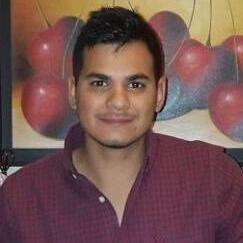
\includegraphics[width=\linewidth]{Foto_CV.png}	%trimming relative to image size

%---------------------------------------------------------------------------------------
%	META SKILLS
%----------------------------------------------------------------------------------------

\cvsection{SKILLS}

\cvskill{Python} {5+ yrs} {1} \\[-2pt]

\cvskill{C++} {7+ yrs} {0.9} \\[-2pt]

\cvskill{LAMP/WAMP} {4+ yrs} {0.85} \\[-2pt]

\cvskill{Google Analytics} {2+ yrs} {0.75} \\[-2pt]

\cvskill{Selenium/Docker} {2+ yrs} {0.75} \\[-2pt]

\cvskill{Django/Dash} {2+ yrs} {0.8} \\[-2pt]

\cvskill{HTML/CSS/Markdown} {5+ yrs} {0.9} \\[-2pt]

\cvskill{Javascript/PHP} {5+ yrs} {0.85} \\[-2pt]

\cvskill{Fortran} {8+ yrs} {0.9} \\[-2pt]

\cvskill{Visual Basic} {8+ yrs} {0.8} \\[-2pt]

\cvskill{R} {5+ yrs} {1} \\[-2pt]

\cvskill{Matlab} {5+ yrs} {1} \\[-2pt]

\cvskill{GitHub} {5+ yrs} {1} \\[-2pt]

\cvsection{CONTACT}

\icontext{MapMarker}{12}{Hermosillo, Sonora}{black}\\[6pt]
\icontext{MobilePhone}{12}{662-364-8525}{black}\\[6pt]
\iconemail{Envelope}{12}{alan.matzumiya@gmail.com}{alan.matzumiya@gmail.com}{black}\\[6pt]
\iconhref{Github}{12}{github.com/alanmatzumiya}{https://github.com/alanmatzumiya}{black}\\[6pt]

%---------------------------------------------------------------------------------------
%	EDUCATION
%---------------------------------------------------------------------------------------- 
\cvsection{LANGUAGES}

\cvskill{Speak English}{80 \%}{0.8} \\[-2pt]
\cvskill{Write English}{90 \%}{0.9} \\[-2pt]

\cvsection{EDUCATION}

\cvmetaevent
{2011 - 2016}
{Chemical Engineering}
{Universidad de Sonora}
{Title obtained when presenting the thesis: \\
	
\href{http://www.repositorioinstitucional.uson.mx/handle/unison/1840}{\textbf{Caracterizaci\'on y evaluaci\'on de las propiedades bioactivas de una mezcla de biocomp\'ositos de hidroxiapatita/$\beta$-wollastonita preparados por el m\'etodo sol gel: sometidos a tratamientos t\'ermicos diferentes}}.}

\cvmetaevent
{2017 - 2019}
{Degree in Mathematical Sciences}
{Universidad de Sonora}
{The objective of obtaining the degree was to develop a solid knowledge in the area of numerical analysis that allowed me to write a thesis on spectral methods making use of Fourier transforms to solve partial differential equations that occur in fluid dynamics. My thesis work, along with the codes that I have developed to understand its computational implementation, can be consulted at:\\

\href{https://github.com/alanmatzumiya/spectral-methods}{\textbf{gh-pages/spectral-methods}}.}

\vfill\null

%---------------------------------------------------------------------------------------
%	CERTIFICATION
%----------------------------------------------------------------------------------------
  

\end{leftcolumn}
\begin{rightcolumn}
%---------------------------------------------------------------------------------------
%	TITLE  HEADER
%----------------------------------------------------------------------------------------
\cvskill{} {\hyperref[spanish]{Read in Spanish}} {1} \\[2pt]
\fcolorbox{white}{darkcol}{\begin{minipage}[c][3.5cm][c]{1\mpwidth}
	\begin {center}
		\HUGE{ \textbf{ \textcolor{white}{ \uppercase{ Alan Daniel Matzumiya Zazueta } } } } \\[-24pt]
		\textcolor{white}{ \rule{0.1\textwidth}{1.25pt} } \\[4pt]
		\large{ \textcolor{white} {I'm Mathematician and Chemical Engineer.} }
	\end {center}
\end{minipage}} \\[14pt]
\vspace{12pt}
%---------------------------------------------------------------------------------------
%	PROFILE
%----------------------------------------------------------------------------------------
\vspace{1mm}
\cvsection{About}
\\
\cvtext{\textbf{Age:} 27 years  \hspace{2mm}  \textbf{Date of Birthday:} 14/09/1992}
\\\\
\cvtext{\textbf{Hometown:} Guaymas, Sonora  \hspace{2mm}  \textbf{Residency:} Hermosillo, Sonora}
\\\\
\cvtext{Thanks to my academic training, it has been possible for me to obtain a wide variety of mathematical tools that allow me to pose and develop problems that require interpretation through models that may be useful depending on their purpose. \\

On my own initiative, and in a self-taught way, I practice in different programming languages, which I have used not only for mathematical purposes but I have also managed to obtain good experiences in web and application development. \\

My main interest is to delve into the area of data analysis, which with my skills in mathematics has been possible for me to explore, interpret and work with data using \textbf{Python}, this being the programming language that I master the most due to the constant practice that I have done for my training as a programmer. \\
\vspace{0.5cm}

\fcolorbox{white}{darkcol}{\begin{minipage}[c][1.4cm][c]{1\mpwidth}
	\begin {center}
		\large{ \textcolor{white} {If you want to know more about me, you can visit my website:}}
		\\[4pt]
		\large{ \textcolor{white} {\hyperlink{https://alanmatzumiya.github.io/}{\textbf{https://alanmatzumiya.github.io}}} }
 	\end {center}
\end{minipage}}
\\\\
Here you can find projects and more detailed information about my academic and professional training.
}

%---------------------------------------------------------------------------------------
%	WORK EXPERIENCE
%----------------------------------------------------------------------------------------
\vspace{5mm}
\cvsection{PROFESSIONAL EXPERIENCE}

\cvevent
{may - jun 2015}
{Professional Practices}
{CFE - Central Ciclo Combinado - Hermosillo}
{\cvlist{
		\item Participation as an observer in environmental audit of the plant.
		\item Proposal for a project to modify a water treatment plant, in order to solve a problem of pressure losses in the pipes that transported the water recovered from the electric power generation process, and that caused spills in a storage tank of Water. 
}}

\newpage
\cvsection{Academic Experience}
\cvevent
{jun 2018}
{Researching in Numerical Methods}
{Instituto de Matem\'aticas, UNAM - Oaxaca de Ju\'arez}
{\cvlist{
		\item The objective of this research, directed by Dr. Francisco Javier Delgado Vences, was to study methods for solving stochastic partial differential equations, which were part of the development of my thesis work to obtain my degree.
		\item Upon completion, I wrote a code in the Python language, which can be found in \hyperlink{https://www.github.com/alanmatzumiya/Paper}{\textbf{github.com/alanmatzumiya/Paper}}, to publish a scientific article on these methods. The article was published as: \\ \href{https://www.researchgate.net/publication/334330862_INITIAL_CONDITIONS_CONTINUITY_OF_A_NUMERICAL_APPROXIMATION_FOR_KOLMOGOROV_EQUATIONS}{\textbf{INITIAL CONDITIONS CONTINUITY OF A NUMERICAL APPROXIMATION FOR KOLMOGOROV EQUATIONS.}}
		\item Based on the above, start building a \textbf{Python Package} whose purpose is to have efficient tools to solve stochastic partial differential equations.
}}

\vfill\null
\cvevent
{2017-2019}
{Programming Courses in Python}
{Universidad de Sonora}
{\cvlist{
		\item I had the opportunity to share my experiences as a programmer through some courses that I organized using as the main tool \textbf{Jupyter Notebook}.
		\item The main idea of these courses was to motivate engineering students to use technology for problem solving.
		\item I am currently working on an educational project that aims to achieve a complete development in the use of the Python language, and that can be consulted by initial or advanced users. Its development can be consulted at:
		\hyperlink{https://www.github.com/alanmatzumiya/python-courses}{\textbf{gh-pages/python-courses}}.
}}

\\

\cvsection{Personal Experience}

\cvtext{
Always motivated for any challenge and to undertake new projects, I took the initiative to experiment with my own distillation equipment, designed to separate the ethanol produced by fermentation. fruits with high sugar content. With this equipment, and with the help of an induced draft cooling system that I managed to build with my knowledge, it allowed me to obtain alcohol with $ 90 $ \% purity without problems. This experience has allowed me to understand in more detail these processes, which in chemical engineering are known as unit operations.
}

% hotfixes to create fake-space to ensure the whole height is used
\mbox{}
\vfill
\mbox{}
\vfill
\mbox{}
\vfill
\end{rightcolumn}
\end{paracol}
\end{document}
